\documentclass[review]{acmsiggraph}
\usepackage{amssymb}
\usepackage{amsmath}
\usepackage{amsbsy}
\usepackage{wrapfig}
\usepackage{soul}
\usepackage{hhline}
\DeclareMathOperator*{\argmin}{arg\,min}

%% editing comment

%\newcommand{\cmt}[1]{\textcolor{red}{\textbf {#1}}}
\usepackage[usenames] {color}
\definecolor{purple}{rgb}{0.4,0.2,0.8}
\newcommand{\cmt}[1]{}
\newcommand{\note}[1]{\cmt{Note: #1}}
\newcommand{\karen}[1]{\textcolor{red}{{Karen: #1}}}
\newcommand{\original}[1]{\textcolor{blue}{{Original: #1}}}
\newcommand{\jie}[1]{\textcolor{blue}{{Jie: #1}}}
\newcommand{\alex}[1]{\textcolor{purple}{{Alex: #1}}}
\newcommand{\greg}[1]{\textcolor{green}{{Greg: #1}}}
\newcommand{\newtext}[1]{#1}
%\newcommand{\newtext}[1]{\textcolor{blue}{#1}}
\newcommand{\eqnref}[1]{Equation~(\ref{eqn:#1})}

%% ignore text
\long\def\ignorethis#1{}

%% abbreviations
\newcommand{\etal}{{\em{et~al.}\ }}
\newcommand{\eg}{e.g.\ }
\newcommand{\ie}{i.e.\ }

%% reference shortcuts
\newcommand{\figtodo}[1]{\framebox[0.8\columnwidth]{\rule{0pt}{1in}#1}}
\newcommand{\figref}[1]{Figure~\ref{fig:#1}}
%\renewcommand{\eqref}[1]{Equation~(\ref{eq:#1})}
\newcommand{\secref}[1]{Section~\ref{sec:#1}}

%% frequently used mathematical structures
\newcommand{\vc}[1]{\ensuremath{\mathbf{#1}}}
\newcommand{\pd}[2]{\ensuremath{\frac{\partial{#1}}{\partial{#2}}}}
\newcommand{\pdd}[3]{\ensuremath{\frac{\partial^2{#1}}{\partial{#2}\,\partial{#3}}}}


% math macros
\newcommand{\vEndEff}{\ensuremath{\vc{d}}}
\newcommand{\vRelMove}{\ensuremath{\vc{r}}}
\newcommand{\sSet}{\ensuremath{S}}


\newcommand{\vControl}{\ensuremath{\vc{u}}}
\newcommand{\vPoint}{\ensuremath{\vc{p}}}
\newcommand{\sSpringCoef}{{\ensuremath{k_{s}}}}
\newcommand{\sDamperCoef}{{\ensuremath{k_{d}}}}
\newcommand{\vHandle}{\ensuremath{\vc{h}}}
\newcommand{\vForce}{\ensuremath{\vc{f}}}

\newcommand{\mTransChain}{\ensuremath{\vc{W}}}
\newcommand{\mRotateTrans}{\ensuremath{\vc{R}}}
\newcommand{\sJoint}{\ensuremath{q}}
\newcommand{\vJoint}{\ensuremath{\vc{q}}}
\newcommand{\mJoint}{\ensuremath{\vc{Q}}}
\newcommand{\mMass}{\ensuremath{\vc{M}}}
\newcommand{\sMass}{\ensuremath{{m}}}
\newcommand{\vGravity}{\ensuremath{\vc{g}}}
\newcommand{\vConstr}{\ensuremath{\vc{C}}}
\newcommand{\sConstr}{\ensuremath{C}}
\newcommand{\vCOM}{\ensuremath{\vc{x}}}
\newcommand{\sGeneralForce}[1]{\ensuremath{Q_{#1}}}
\newcommand{\vStateVar}{\ensuremath{\vc{y}}}
\newcommand{\vControlVar}{\ensuremath{\vc{u}}}
\newcommand{\argmax}{\operatornamewithlimits{argmax}}
\newcommand{\tr}[1]{\ensuremath{\mathrm{tr}\left(#1\right)}}




%%%%%%%%%%%%%%%%%%%%%%%%%%%%%%%%%%%%%%%%%%%%%%%%%%%%%%%%%%%%%%%%%%%
%
% Here are a bunch of macros, mostly for math.
%
%%%%%%%%%%%%%%%%%%%%%%%%%%%%%%%%%%%%%%%%%%%%%%%%%%%%%%%%%%%%%%%%%%%

\renewcommand{\choose}[2]{\ensuremath{\left(\begin{array}{c} #1 \\ #2 \end{array} \right )}}

\newcommand{\gauss}[3]{\ensuremath{\mathcal{N}(#1 | #2 ; #3)}}

\newcommand{\pctab}{\hspace{0.2in}}
\newenvironment{pseudocode} {\begin{center} \begin{minipage}{\textwidth}
                             \normalsize \vspace{-2\baselineskip} \begin{tabbing}
                             \pctab \= \pctab \= \pctab \= \pctab \=
                             \pctab \= \pctab \= \pctab \= \pctab \= \\}
                            {\end{tabbing} \vspace{-2\baselineskip}
                             \end{minipage} \end{center}}
\newenvironment{items}      {\begin{list}{$\bullet$}
                              {\setlength{\partopsep}{\parskip}
                                \setlength{\parsep}{\parskip}
                                \setlength{\topsep}{0pt}
                                \setlength{\itemsep}{0pt}
                                \settowidth{\labelwidth}{$\bullet$}
                                \setlength{\labelsep}{1ex}
                                \setlength{\leftmargin}{\labelwidth}
                                \addtolength{\leftmargin}{\labelsep}
                                }
                              }
                            {\end{list}}
\newcommand{\newfun}[3]{\noindent\vspace{0pt}\fbox{\begin{minipage}{3.3truein}\vspace{#1}~ {#3}~\vspace{12pt}\end{minipage}}\vspace{#2}}



\newcommand{\key}{\textbf}
\newcommand{\fun}{\textsc}

%\def\shortcite{\def\citename##1{}\@internalcite}


% Local Variables:
% TeX-master: "paper"
% End:

\TOGonlineid{0000}



\TOGvolume{0}
\TOGnumber{0}
\TOGarticleDOI{1111111.2222222}
\TOGprojectURL{}
\TOGvideoURL{}
\TOGdataURL{}
\TOGcodeURL{}

\title{Simulating Animations of Human Dressingpwd
}


\author{Alex Clegg \and Jie Tan \thanks{e-mail: jtan34@gatech.edu} %
\and Greg Turk \\ \\ Georgia Institute of Technology %
\and C. Karen Liu}

\pdfauthor{Alex Clegg, Jie Tan, Greg Turk, C. Karen Liu}

%% Keywords that describe your work.

\keywords{Bicycle simulation, balance control, reinforcement learning, neural networks.}


\begin{document}

%% The ``\maketitle'' command must be the first command after the
%% ``\begin{document}'' command. It prepares and prints the title block.

%%\teaser{
%%  \includegraphics[width=\textwidth]{images/HSwing}
%%  \caption{An H-shaped character does its morning exercises.}
%%  \label{fig:HSwing}
%%}
\maketitle

%% Abstract section.

\begin{abstract}
%Dressing is one of the most common activities in human society. Perfecting
the skill of dressing can take an average child three to four years of
daily practice. The challenge is primarily due to the combined difficulty
of coordinating different body parts and manipulating soft and deformable
objects (clothes). We present a technique to synthesize human dressing by
controlling a human character to put on an article of simulated clothing.
We identify a set of \emph{primitive actions} which account for the vast
majority of motions observed in human dressing. These primitive actions
can be assembled into a variety of motion sequences for dressing different
garments with different styles. Exploiting both feed-forward and feedback
control mechanisms, we develop a dressing controller to handle each of the
primitive actions. The controller plans a path to achieve the action goal
while making constant adjustments locally based on the current state of
the simulated cloth when necessary. We demonstrate that our framework is
versatile and able to animate dressing with different clothing types
including a jacket, a pair of shorts, a robe, and a vest. Our controller
is also robust to different cloth mesh resolutions which can cause the
cloth simulator to generate significantly different cloth motions. In
addition, we show that the same controller can be extended to assistive
dressing.

% Because the human dressing motion is difficult to animate or motion capture, the input motion does not need to be exact or complete (a few keyframes or pretend-dressing mocap). We develop a feedback controller that takes into account the state of cloth

\end{abstract}

\begin{CRcatlist}
  \CRcat{I.3.7}{Computer Graphics}{Three-Dimensional Graphics and Realism}{Animation};
  \CRcat{I.6.8}{Simulation and Modeling}{Types of Simulation}{Animation}.
\end{CRcatlist}

%% The ``\keywordlist'' command prints out the keywords.
\keywordlist
\copyrightspace

% 
\section{Introduction}
\vspace{-0.1 in}
% \karen{Very high level comments: 1. Most problems mentioned in the
%   second paragraph are based on the assumption that animators use
%   physics simulation to generate cloth motion. We might want to
%   establish this assumption first by describing a general or
%   reasonable approach for creating cloth/human motion. 2. We want to
%   explicitly state the input of our system. 3. Our problem can be
%   viewed as path planning. It's very difficult because the cloth keeps
%   moving and the human body can easily self-collide. Further, we are
%   facing a very unique problem regarding human/cloth collision. Unlike
%   most navigation problems, our goal is not to avoid colliding with
%   cloth. Instead, our goal is to embrase and utilize contacts to
%   change the state of clothes in order to achieve the task. }

This paper describes a system for animating the activity of putting on
clothing.  Dressing is one of the most common activities that each of us
carries out each day.  Scenes of dressing are also common in live-action
movies and television.  Some of these scenes are iconic, such as the
``jacket on, jacket off'' drill in The Karate Kid (2010 version) or
Spiderman pulling his mask over his head for the first time.  Such
dressing scenes are noticeably absent in computer animated films.  Despite
the importance of dressing in our lives and in film, there is as yet no
systematic approach to animating a human that is putting on clothing.

% Mr. Rogers putting on his cardigan sweater in the children’s TV show,
% Mrs.  Robinson slipping on her stockings in The Graduate.
%
% The trailer for The Incredibles shows how far a computer animator will
% go to avoid showing a character pulling on their clothes.  

Our goal is to provide a system that will allow an animator to create
motion for a human character that is dressing.  We want the animator to
have a high degree of control over the look of the final animation.  To
this end, we desire a system that allows the user to describe the dressing scene as a sequence
of high-level actions.  Also, we would like our system to
accept approximated human motion, in either the form of keyframes or
motion capture, as reference for styles or aesthetics.  Thus the input from
the animator for a given dressing scene consists of: a character model,
a garment, a sequence of dressing actions, and reference
motions for the character. In order to create animation that is
physically plausible, we made the choice to use physical simulation of
cloth to guide the garment motions. By using cloth simulation, the
human figure, made of a collection of rigid segments, can interact
with the cloth in a natural manner.
 
% Our system takes these inputs from the animator and creates a physically
% realistic looking animation.  In order to create animation that is
% physically plausible, we made the choice to use physical simulation of
% cloth to guide the garment motions.  By using cloth simulation, the motion
% of the character affects the cloth motion in a natural manner.  We
% represent our human figures as a collection of rigid segments that are
% connected by joints.

% People use a wide variety
% of clothing types, including: shirts, pants, underwear, dresses, skirts,
% socks, shoes, hats, gloves, vests, jackets, and sweaters.

The essence of animating the act of dressing is modeling the
interaction between the human character and the cloth.  The human's motion
must adapt to the motion of the cloth, otherwise problems occur such as the
clothing slipping off or a hand getting stuck in a fold.  We often take
for granted the complex set of motions that are needed to put on our
clothes.  The seemingly simple act of putting on a jacket requires a
careful coordination between the person and the jacket.  Unconsciously we
make constant adjustments to our hand's position when inserting it into
the jacket's sleeve.  We hold our body at an angle to keep a sleeve from
sliding off our shoulder.  After putting on the first sleeve, we may use
any of several strategies to get our hand behind our back and within reach
of the second sleeve.  A system for animation of dressing must address
these kinds of complexities.

We have found that a small set of \emph{primitive actions} account for the vast
majority of the motions that a person goes through to put on an article of
clothing.  The approach that we take to dressing is to first have the
animator assemble a desired dressing motion from a small number of such
actions.  These actions include placing a hand or foot through an opening,
pulling the garment onto a limb, and stretching out a limb after it has
been positioned in the clothing.  Once this sequence of actions has been
assembled, producing the dressing animation can proceed.  The system steps
forward in time, updating the cloth's position through simulation.  The
character's motion during each of the actions are guided by optimization
and planning in order to satisfy the requirements of a given
action. The system adjusts the character's pose to match the end of one
action to the start of the next. Some portions of a dressing sequence do
not require the character to react to the cloth, and such segments can follow
the provided keyframe or motion capture data.

To a large degree, the problem that a dressing animation system must solve
is a form of \emph{path planning}. The character's body parts must move in coordination to
complete the task while preventing self-intersection and the
character must move in and around the cloth in such a way that the garment
ends up properly on the person. However, the dressing problem has a
few unique challenges which are not addressed by standard path planning
algorithms. Unlike typical path planning that avoids
collisions, contact between the body parts and the cloth is to be
expected. In fact, \emph{utilizing} contact to expand the opening of a folded
sleeve or fixate a part of cloth on the body is crucial for
successful dressing.

% To a large degree, the problem that a dressing animation system must solve
% is a form of \emph{path planning}.  First, the character's motion must not
% cause self-intersection between body parts.  We use several techniques
% for avoiding such collisions between body parts.  Moreover, the character
% must move in and around the cloth in such a way that the garment ends up
% properly on the person.  Some actions specifically require the character
% to react to the motion of the cloth.  Consider the case of trying to put a
% foot into the opening for one leg in a pair of pants.  Our system
% constantly adjusts the motion of the character's foot so that it draws
% closer to the opening without getting tangled in the cloth.  We accomplish
% this by using visibility information about the cloth to provide feedback
% that controls the limb's motion.  Note that this is not the typical form
% of path planning that would avoid colliding with the cloth.  Contact
% between the person and the cloth is to be expected.

Using our action-based dressing system, we have produced a variety of
animations of a character that is putting on various types of clothes.
This includes putting on a jacket, pulling on pants while sitting, putting
on pants while standing, dynamically swinging on a vest, and having one character assist another in putting on a robe.



% \section{Related Work}

Interacting with surrounding humans or objects is an important research problem in character animation. Much previous research focused on close range interaction, which involves many challenging problems, such as collisions handling \cite{Ye:2012}, spatial constraints solving \cite{Ho:2010:SRP}, and path planning \cite{Kallman:2003,Yamane:2004:SAH,Bai:2012:SCO}. These existing techniques generated interesting animations beyond what simple forward simulation or keyframe interpolation can achieve. However, most methods assumed that the character interacts with humans or objects made of rigid bodies. Ho and Kumar \shortcite{Ho:2009:CMS} introduced a technique to interact with deformable bodies using topology coordinates, in which the topological relationship of the character's body and the environment can be easily controlled.

- Spatial Relationship Preserving Character Motion Adaptation
Path planning
- Synthesis of Concurrent Object Manipulation Tasks
- Planning collision-free reaching motions for interactive object manipulation and grasping
- Synthesizing animations of human manipulation tasks


Hand manipulation with soft objects
- Coupling Cloth and Rigid Bodies for Dexterous Manipulation
 Robotic cloth manipulation

Dexterous manipulation is a broad research area that has a vari- ety of applications in computer graphics and robotics. Although a precise definition is still open to interpretation, dexterous manipu- lation is typically defined as the use of multiple fingers to achieve a desired object configuration. In computer graphics, researchers have shown that intricate control strategies, such as finger gaiting [Ye and Liu 2012], rolling/sliding [Liu 2009; Bai and Liu 2014], or grasping/regrasping [Pollard and Zordan 2005; Kry and Pai 2006; Zhao et al. 2013; Wang et al. 2013], can be physically simulated on an anthropomorphic hand model. However, one of the most im- portant assumptions these techniques make is that the manipulated objects are rigid bodies with only six degrees of freedom.Manipulating deformable objects is a more challenging problem due to more degrees of freedom and more complex collision phenomena. Researchers in robotics have studied the problems of manipulat- ing fabric, cables, foam rubber, or sheet metal [Kosuge et al. 1995; Wu et al. 1995; Fahantidis et al. 1997; Osawa et al. 2007; Bersch et al. 2011; Miller et al. 2012]. Many previous approaches enhance control and planning algorithms by using simulation techniques to estimate the state of the deformable objects. For example, robotics researchers used a cloth simulator to approximate the contour of the clothes being folded by a PR2 robot [Cusumano-Towner et al. 2011]. Because the interaction between the robot hands and the cloth was relatively simple (i.e. grasping only), their simulation ap- plied position constraints to pin the cloth in the air instead of sim- ulating the hands. Our work aims to simulate the hands, the cloth, and their effects to each other realistically. We show that with a more accurate simulation routine, a wide variety of manipulation strategies can be achieved.


Cloth control without hands
- Manipulation of Flexible Objects by Geodesic Control
- Harmonic Parameterization by Electrostatics
Wojtan
Jernej


Papers that demonstrate dressing:
- Character Motion Synthesis by Topology Coordinates: They generated keyframes in topology coordinates and interpolate motion. The character does not respond to the state of the clothes. No autonomous control. They demonstrated that a character stretching the arms out of a piece clothes wrapped around it using keyframes. 
- Harmonic Parameterization by Electrostatics
- Clothing manipulation, Igarashi


Cloth sim interacting with rigids
- Coupling Cloth and Rigid Bodies for Dexterous Manipulation

% \section{Overview}

\begin{figure}
  \centering
  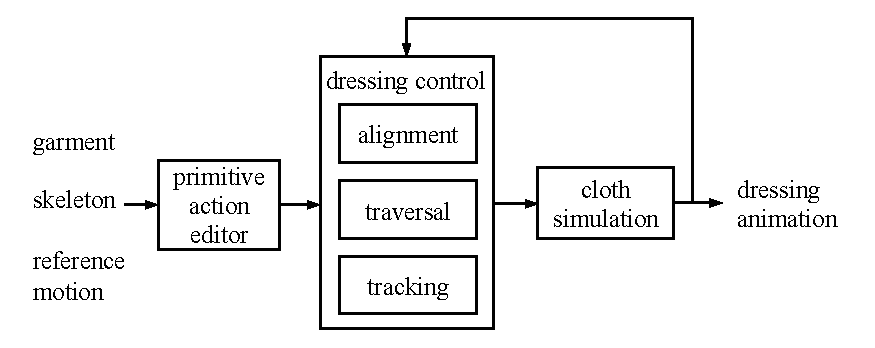
\includegraphics[width=3.3in]{images/overview}
  \caption{The overview of our system.}
  \label{fig:overview}
\end{figure}

\begin{table}
  \centering
  \begin{tabular}{|l|l|}
    \hline
    Action & Description \\
    \hline
    Grip(RH, $\vc{f}_{1}$) & Grip the colar feature $\vc{f}_1$  with the right hand.\\
    Track($\hat{\vc{q}}(t)$, $T_1$) & Track the reference motion $\hat{\vc{q}}$ for $T_1$ seconds.\\
    Align(LH, $\vc{f}_{2}$) & Align the left hand with the armhole $\vc{f}_2$.\\
    Drag(RH, $\{B_i\}$) & Drag the cloth along the left hand $B_1$, the left\\
    &                      arm $B_2$ and the left shoulder $B_3$.\\
    Release(RH) & Release the cloth from the right hand.\\
    Idle($T_2$) & Idle for $T_2$ seconds.\\
    Track($\hat{\vc{q}}$(t), $T_3$) & Track the reference motion $\hat{\vc{q}}$ for $T_3$ seconds.\\
    Align(RH, $\vc{f}_{3}$) & Align the right hand with the right armhole $\vc{f}_3$.\\
    Stretch(RH) & Stretching the right hand into the sleeve.\\
    Track($\hat{\vc{q}}$(t), $T_4$) & Track the reference motion $\hat{\vc{q}}$ for $T_4$ seconds. \\
    \hline
  \end{tabular}
  \caption{An example action queue for dressing the upper body of a character with a jacket.}
  \label{table:actionQueue}
\end{table}


We have designed a system that allows a virtual human character to put on various types of garments. Our system consists of three main components: action queue, dressing control the cloth simulation.
At each step, our system fetches an action from the queue,
executes its corresponding dressing controllers and simulates the physics of the cloth. Figure \ref{fig:overview} illustrates the main components of our system. 
Given a piece of garment, a character and a reference dressing motion, our system allows a user to decompose the entire
dressing sequence into a queue of high level actions. For example, putting an arm into a sleeve involves \emph{aligning} the hand with the armhole and
\emph{dragging} the cloth from the wrist to the shoulder. 
Table~\ref{table:actionQueue} shows complete action queue for putting on a jacket.
For each action, we design kinematic dressing controllers that determine desired end effector positions based on the current cloth states, solves IK problems for full body poses and plans a collision-free joint path to fulfill the action. 






% \input{simulation}
% \input{control}
% \section{Results}
\begin{table}[b]
  \centering
  \begin{tabular}{|l|c|c|c|c|c|}
    \hline
    examples 		& cloth 	& act- 	& anim	& sim 		& control \\
                    & triangles & 	ions& time 	& time 		& time \\
    \hline
    jacket 			& 23.2k  	& 10	& 18s 	& 30h23m	&  14m  \\
    jacket (low res)& 2.7k		& 10	& 18s	& 2h58m		& 1m \\
    shorts (sitting) 	& 14.9k 	& 10	& 16s 	&  8h41m 	& 4m \\
    shorts (standing)	& 14.9k 	& 10	& 15s	&  7h52m	& 3m \\
    vest 			& 6.57k		& 14	& 13s	&  3h53m	& 1m   \\
    robe 			& 31.7k 	& 11	& 14s	& 20h40m	& 19m  \\
    \hline
  \end{tabular}
  \caption{Parameters and performance of the examples. cloth triangles: the number of elements in cloth simulation. Actions: number of actions. Anim time: wall clock time (in seconds) of the dressing animation. Sim and control times are the total times for the cloth simulation and our control functions respectively.}
  \label{table:data}
\end{table}


In this section we describe the results of our system. We chose four different types of garments from the Berkeley Garment Library, edited them to meet our needs, and put them on the character using different styles. Please watch the accompanying video for the dressing animations. Our system was implemented in C++. We used DART \cite{Liu:2012:STM} for human character modeling and ARCSim \cite{Narain:2012:AAR} for cloth simulation. We used a denim material profile with 3-4x thickening to simulate layered clothing articles. The examples were run on a desktop workstation with a 4-core 3.7 GHz CPU and 8 GB of memory. The typical running time of a dressing example is several hours to a day. The cloth simulation is the most time-consuming part and takes significantly longer than control. The parameters and performance data of our examples are summarized in Table
 \ref{table:data}. 


\paragraph{Jacket.} Figure~\ref{fig:jacket} shows a character putting on a
jacket using a common style: Put the left arm in its sleeve, swing the right arm to the back, find the hanging sleeve, and stretch the arm into it. The reference human motion for this style is made up of six keyframes. As shown in the video, dressing by directly playing back the reference motion without any feedback control fails to put on even the first sleeve. After gripping the collar of the cloth, our system first tracks the reference motion to a particular keyframe and then performs an alignment action. The character aligns his left hand with the corresponding armhole. Once the alignment is successful, the traversal action is executed. The character uses his right hand to drag the cloth up the length of the left arm. At the end of traversal, the right hand reaches the shoulder and releases the cloth. The character then swings his right arm to the back by tracking the reference motion. The second alignment phase begins when the character's right hand starts to search for the opening of the sleeve. This alignment phase is more challenging because the target armhole is completely occluded by multiple layers of cloth. The alignment action gradually finds better intermediate goals that are closer to the target feature and guides the hand to wiggle through the cloth folds towards the goal. 

In the jacket example we observed interesting emergent behavior, such as a natural exploratory gesture that is often used by humans to sort out the tangled cloth in dressing. Furthermore, the hand operates within a tight space between the pelvis and the hanging cloth during alignment. Without the collision-free IK, the hand or arm would penetrate the torso before aligning with the armhole. After the alignment, the character uses the traversal action to stretch the right arm into the sleeve and then tracks the reference motion until the jacket is completely on the body. 

A common challenge in cloth simulation is that the simulation may produce
drastically different motions if the resolution of the cloth changes. To
test the robustness of our system, we used the same actions to put on a
low resolution jacket with approximately 10x fewer triangles. Our system
was able to automatically adapt to the change in resolution and the
resulting differences in cloth motion without any manual tuning. Note that
the more coarse resolution cloth has fewer wrinkles and folds.  A
consequence of this is that the lower resolution jacket has a less occluded
armhole, so the right hand alignment phase is shorter in this sequence.

\paragraph{Vest.} We simulated putting on a vest in a more dynamic style (Figure~\ref{fig:vest}). We chose this example to demonstrate that using a small set of primitive actions, our system is able to put on a garment in a different style by using a different reference motion. Tracking the motion captured reference, the character swings the vest around his neck, then aligns the left hand with the corresponding armhole while the vest is swinging in mid-air. This alignment shows that our feedback control is robust and able to align not only with a target feature that is occluded by layers of cloth, but also with one that is moving quickly. Once the first arm is dressed, the right hand is aligned with the second armhole and stretches into it. 

\begin{figure*}[!t]
  \centering
  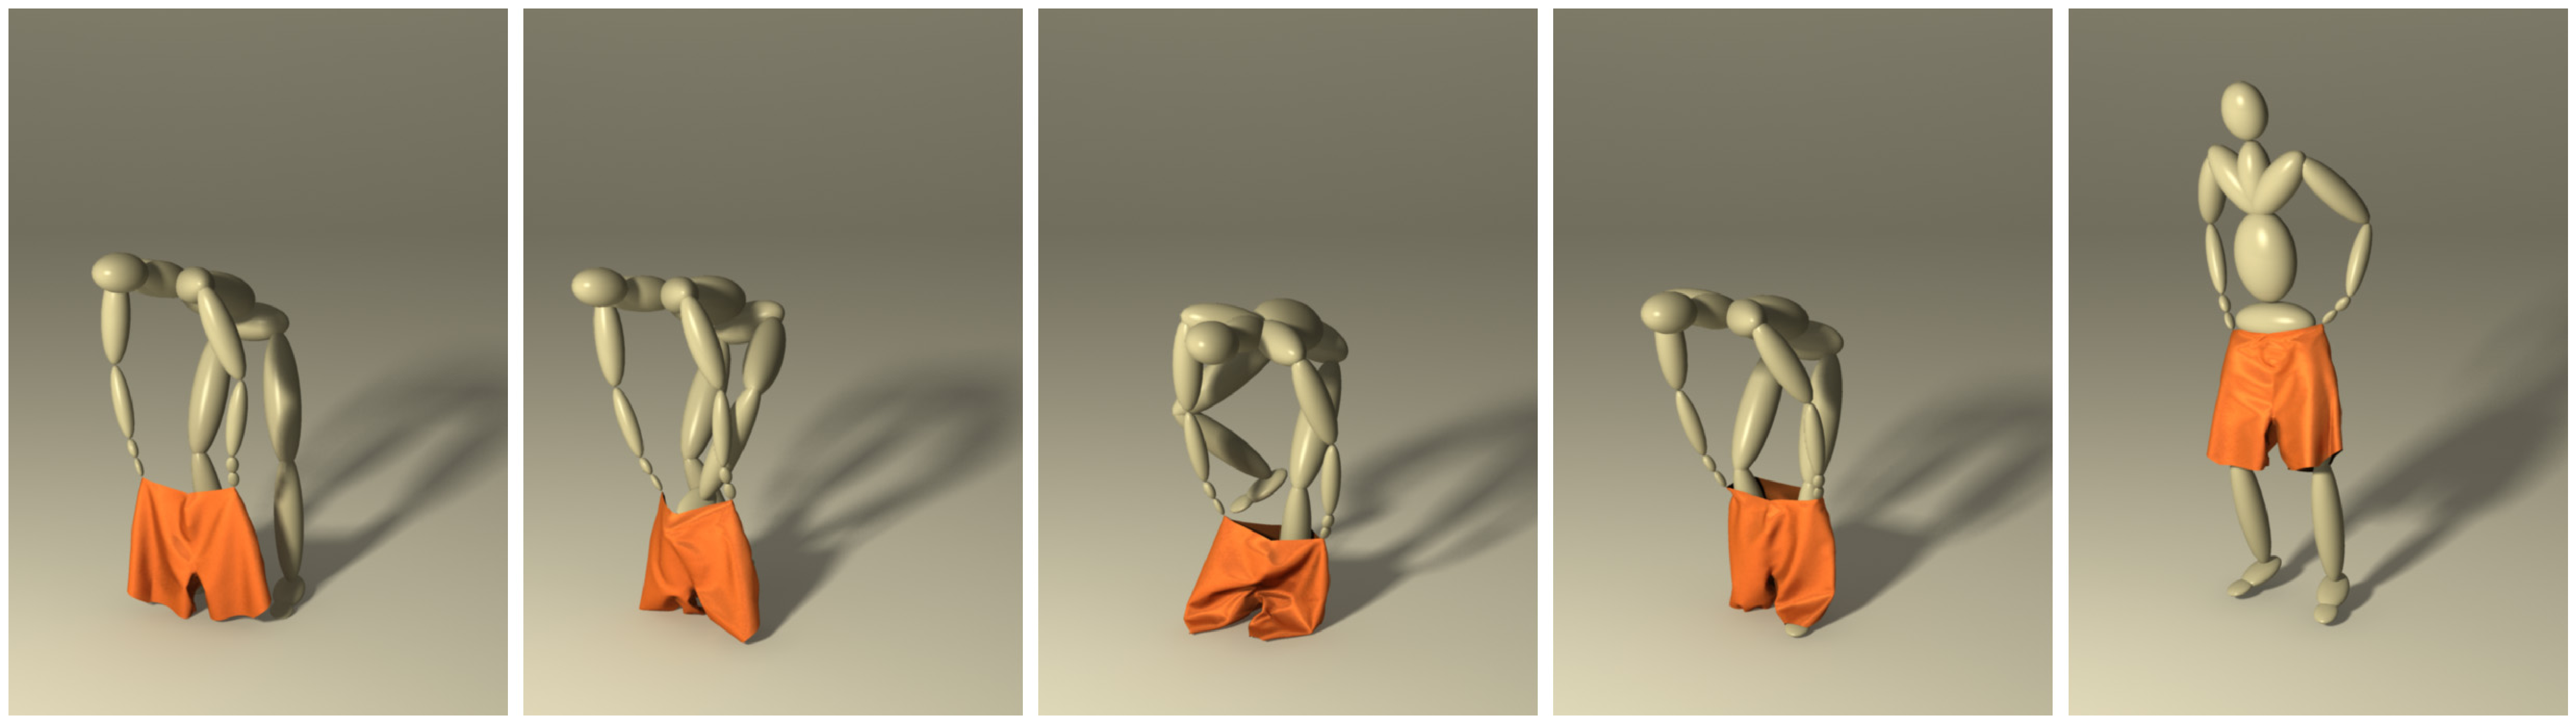
\includegraphics[width=\textwidth]{images/shortsStanding}
  \caption{A character puts on a pair of shorts in a standing pose.}
  \label{fig:shorts2}
\end{figure*}

\begin{figure*}[!t]
  \centering
  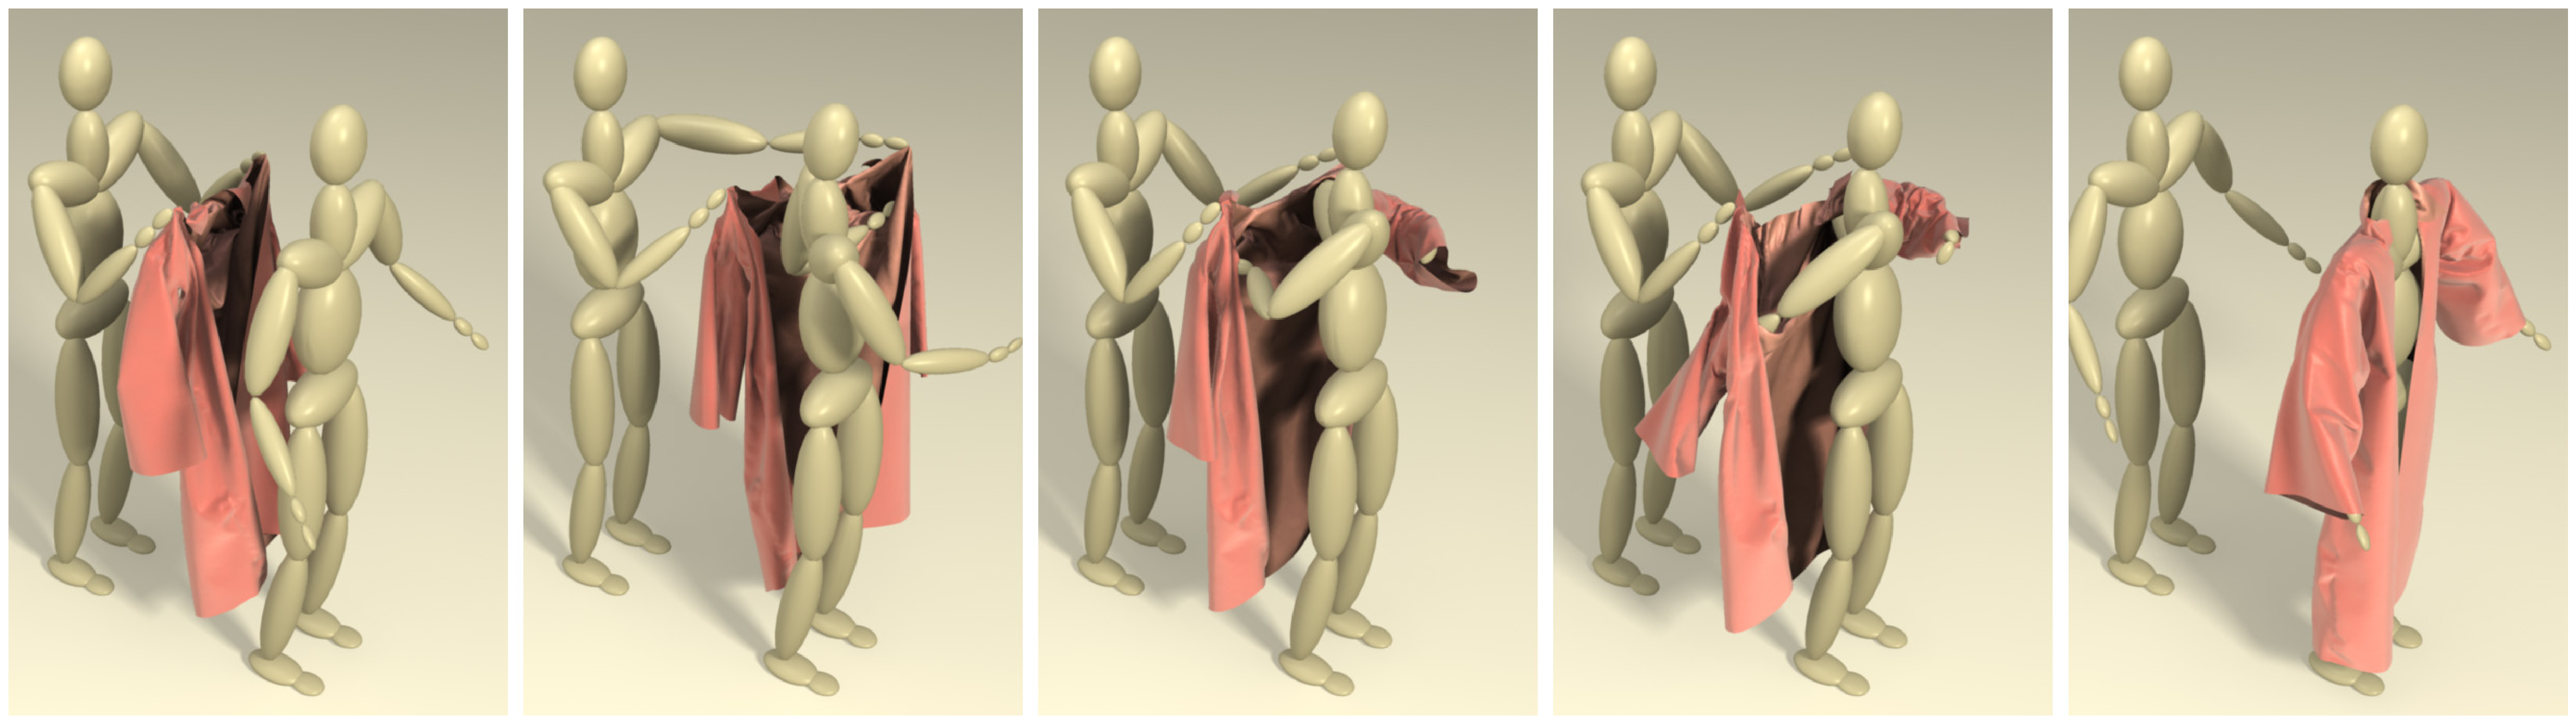
\includegraphics[width=\textwidth]{images/robe}
  \caption{A character puts on a robe with the help from another character.}
  \label{fig:robe}
\end{figure*}

\paragraph{Shorts.} Figure~\ref{fig:shorts1} demonstrates a character that
is putting on a pair of shorts in a sitting position. We used a motion
capture sequence as the reference motion in this example. The character
grips the waistband and leans forward by tracking the reference motion. He
first aligns his left foot with the waistband and then aligns it with the
bottom of the shorts' left leg. Similar alignment actions are applied to
the right foot. Once both feet are aligned with the desired features, the
character follows the reference motion to stand up and pull up the shorts.
The accompanying video shows that without the feedback control, the
character fails to put the feet into the shorts and ends up not wearing
the pants.

We also tested the generality of our system by using a different reference motion, in which we mocaped a person that is putting on a pair of shorts in a standing position. Despite the different style, we were able to reuse the action queue from the sitting shorts and successfully dress the lower body of the character (Figure \ref{fig:shorts2}).

\paragraph{Robe.} To show that our system can be used outside of the realm of self-dressing, we applied our method to an assisted dressing scene in which one character aids another in putting on a robe (Figure \ref{fig:robe}). The reference motion for this scene consists of five keyframes. First, the dressing character tracks the reference motion, twisting to the left and aligning his left hand with the armhole. After he straightens his arm into the sleeve, the assistant releases the cloth from his left hand. Dressing the second arm is similarly performed with both characters tracking to a pre-alignment position whereupon the dressing character aligns and straightens his arm and the assistant releases the sleeve. Note that in this example, the dressing control is only performed on the dressing character while the motion of the assistant is pre-scripted. It would be interesting future work to simulate and control both characters in an assisted dressing task.

% \input{discussion}
% \section{Conclusion}

We have presented a system that allows an animator to create motions
of people that are dressing.  By providing reference motion and an
action sequence, an animator has a fine degree of control over the
method and the style that a character uses to put on a garment.  We
have demonstrated the use of our method in creating a variety of
dressing animations, including putting on a jacket, a vest, pants
while sitting, pants while standing, and assistance in putting on a
robe.  They key technical aspects of our system are collision-free
inverse kinematics, path planning for limbs, and end effector path
planning using visibility feedback from the cloth. \karen{Probably
  want to revise the last sentence according to our recent discussion.}

There are several avenues for future work on animated dressing.  One
possibility is to incorporate dexterous manipulation of the cloth with our
current system.  Such an augmented system would allow a hand to properly
grip a sleeve, instead of ``gluing'' the hand to a portion of the cloth as
we currently do.  Another important aspect of dexterous manipulation that
we have not explored is the use of hands in fastening the garments, as is
needed to use buttons, zippers and laces.  As suggested in the Limitations
section, we might want a system that can figure out a high level dressing
strategy for a newly presented garment.  Such a system would likely need
to do some form of search across a variety of possible dressing
strategies.  There are potential improvements to cloth simulation that
could lead to higher quality dressing animation.  Current cloth simulators
do not handle multiple layers of cloth well, such as putting on a jacket
over a shirt.  The ability to handle tight contact between cloth and
the human figure would also increase the range of possible dressing
simulations.



\bibliographystyle{acmsiggraph}
\bibliography{template}

%\section{Appendix}

\jie{This should go to supplementary material.}
\begin{table}
	
  \begin{tabular}{|l|l|l|l|}
    \hline
    jacket 				& shorts 		& vest 			& robe \\
    \hline
    grip (right) 		& grip (right)	& grip (right)	& grip (left 2) \\
    track 				& grip (left)	& grip (left) 	& grip (right 2) \\
    align (left) 		& track 		& track 		& track\\
    Drag (left)			& align (left)	& release(left)	& align(left)\\
    release(right) 		& align (left)	& align (left)	& track\\
    track 				& track			& track			& release(left 2)\\
    align (right) 		& align (right) & grip (left)	& track\\
    Stretch	(right)		& align (right)	& release (right)& align (right)\\
    track 				& track 		& track			& track\\
    idle				& idle			& align(right)	& release\\
    					&				& release (right)& track \\
    					&				& Stretch (right)& \\
    					&				& track 		&  \\
    					&				& idle			& \\
    \hline
  \end{tabular}
  \caption{Action queue for various dressing scenes with only active actions.}
  \label{table:data}
\end{table}

\end{document}
